\section{The finding of Meridian Way}
\begin{marginfigure}
\begin{tikzpicture}
\node [name-dest] (box){%
    \begin{minipage}{0.80\textwidth}
     \begin{itemize}
    \item Rhys Tyers
    \item Tanguy Racine
    \end{itemize}
    \end{minipage}

};
\node[fancytitle, right=10pt] at (box.north west) {Meridian Way};
\end{tikzpicture}
\end{marginfigure}

The quest of finding a lower entrance to the system is without any doubt a noble one and hasn't been completed as I write these lines. The \passage{Jetstream} extension of the system was spearing south, well away from the main tangle of passages that make up \passage{Sysmig}. Less than 400m to the surface, southwards and upwards, the chances of ending the push by popping out onto the sunlit forest floor were as good as any. In fact, they were better than that: the serendipitous discovery of \passage[cave]{Coincidence Cave} earlier in the week (\vref{sec: coincidence cave}) had revived the belief that the entrance might exist. A draughting hole on the surface, the alignment of a large surface canyon with the underground passage. What are the odds?

\begin{pagefigure}
\checkoddpage \ifoddpage \forcerectofloat \else \forceversofloat \fi
\centering
\frame{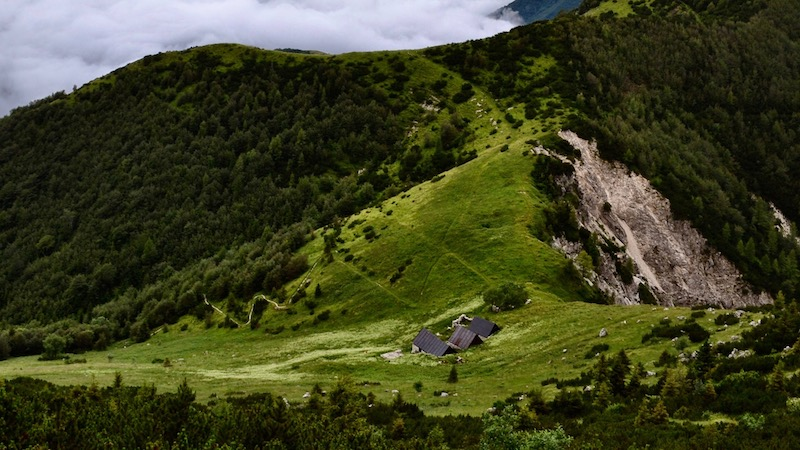
\includegraphics[width=\textwidth]{images/2015/tanguy-meridian-2015/kal-clouds.jpg}}
\caption{Where we hoped to meet the surface, somewhere in the lush landscape below the \protect\passage{Sheperd's Hut} (\protect\passage{Planina Na Kalu}) --- Rhys Tyers}
\label{planina na kalu}
\end{pagefigure}

Rhys and I checked in at camp \passage{X-Ray} for three nights and two pushing days. \bignote{The ambitious plan was to set off smokers at the pushing front, while a party waited for the appearance of red smoke at the surface} thus proving the passage was connected. This would bring us much needed closure.

After an early start, Rhys and I set off from camp, along the now familiar Kamikaze extensions, the long silent passages of \passage{Atlantis}. To our left, the offshoot of \passage{We're Not Alone} beckoned. With the limit of exploration so close, we could not help but have a look at it, to assess the feasibility of pushing the lead. The passage first trended east and bent to the south sharply before turning into a flat cleanwashed crawl. With the ceiling coming to meet the floor to a tight, awkward flat out squeeze, it was no wonder the lead had been left unpushed. Passage could be seen continuing beyond, but we left it at what it was: a lead for thin people.

It was almost eleven o'clock, we had been caving at a good pace, and the front was half an hour away. We pressed on, past the boulder field leading to \passage{Sic Semper Tyrannis}, along passages named and trodden since the previous year only. At the main junction to \passage{Jericho}, we turned left, upwind, up the rift. I passed the down climb to \passage{Squidgy Goodness} where the corpse of the Creature was, and up the ropes Gergely had rigged in 2014. Rhys disappeared down the next pitch, which was the beginning of \passage{Jetstream} and showed me the way up the climbs.

\begin{figure*}[t!]
\checkoddpage \ifoddpage \forcerectofloat \else \forceversofloat \fi
\centering
\frame{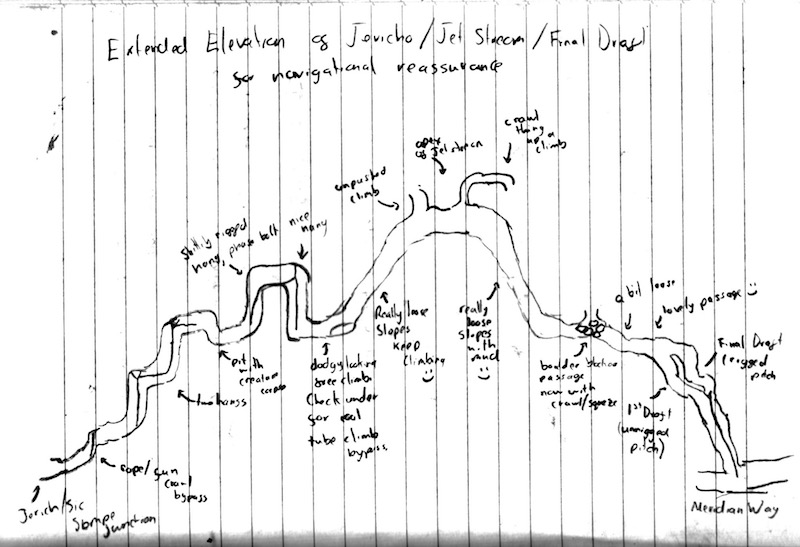
\includegraphics[width=\textwidth]{images/2015/tanguy-meridian-2015/extended_elevation_south.jpg}}
\caption{The hand survey of the southern extensions, drawn in the Underground Camp logbook --- Rhys Tyers}
\label{Notebook}
\end{figure*}

At the very apex of surveyed passage of \passage{Jetstream}, the rift split into two routes. One was continuing directly upwards in the same fashion as the ten metre pit we'd just free climbed. The convenient ledges that had brought us this far disappeared quickly and it was deemed unsafe without a rope. Glory would have to wait. Instead, we slid down the slanting rift continuation, down the scree slope to a boulder choke. When \bignote{faced with the pushing front, crowbar in hand and with a clear idea of what was to be done, a smile crept on my face}: that was precisely what I'd signed up for, thrilled by the countless possibilities of what lay beyond!

I levered a block of limestone out of the choke, then pushed two others to the side, and the way on was clear. I wriggled forward, both hands forward, getting a grip on the boulders on the other side and sat, looking, silent. Rhys followed quickly.

Grinning at the continuation, we stepped off to find the lower entrance. For about 30m the dream was on because the cave didn't change nature: it remained an unstable chossy bedding plane descent. I heard Rhys commenting on the lack of easy walking passage.

Almost as an answer to our expectations, the passage opened up almost instantly into a walking, dry, vadose passage and better still, led to a junction! Rhys stepped to the right, I to the left. The passage on the left twisted down and up before resuming its southern course, but the fault control, pervasive in that part of the cave meant it was going down, ever so slightly towards the west. `Of course!' I thought. The faults were dipping west, and we were locked on their plane. \bignote{Occasionally I would point out to Rhys where the fault planes were exposed, they were beautifully smooth}.

When the passage wormed its way to the top of a sloping pitch, we knew it was almost a game over for us. We were too deep, or not far enough south to intercept the surface. Descending the pitch meant we had to find more horizontal distance! Still, we decided to descend, first by free climbing the 55$^{\circ}$  slope, using the various ledges covered by white sand. About 5 metres down, the slope increased and it dawned on us that we would have to bolt it.

Having left our rope and bolting kit at the start of the squeeze, we doubled back to retrieve them and set about driving the anchors for a Y-hang. I put in the first one, far above the pitch head as it was easier for a left-handed person. Rhys put in the other, and rigged his descender. Down he went until he reached the stopper knot. \bignote{The end of the pitch was in sight, but the rope was a good ten metres short}. It would also need to be deviated.

We considered our options: there was rope at the junction at the start of \passage[junction]{Jericho}, but the horror of \passage{Jetstream} (\passage{Penitence}-like crawl, loose climb, muddy slope etc.) had to be passed again and again. As it was approaching two o'clock, we resolved to abandon the plan to set off the smokers and instead to simply reach the bottom of the pitch and see what was there.

At \passage[junction]{Jericho} junction, after a soupy-fishy-couscous mix, we retrieved the longer rope and turned back towards the pushing front. At the pitch head, I descended slowly, watching the rope carefully to avoid rub points on the various ledges. I had put a deviation two thirds of the way down which ended up swallowing 5 metres of green tape. This done, my feet touched the floor once more on virgin passage. I stayed silent as Rhys descended.

\begin{map}[t!]
\checkoddpage \ifoddpage \forcerectofloat \else \forceversofloat \fi
\centering
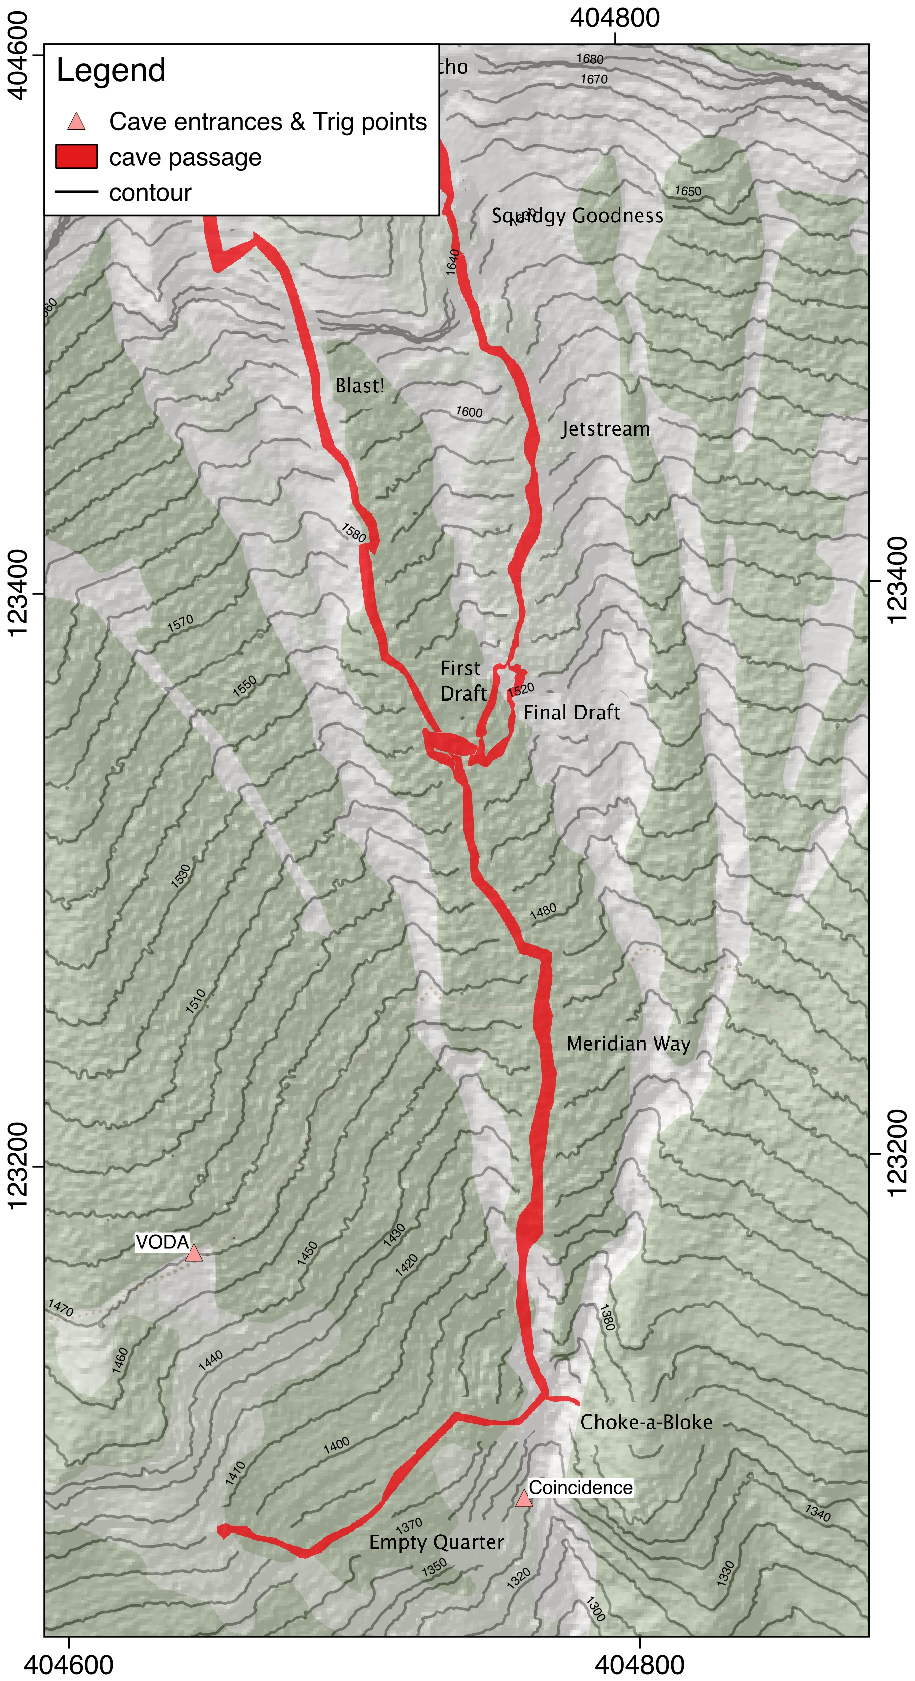
\includegraphics[width=\textwidth]{images/2015/tanguy-meridian-2015/meridian_map.pdf}
\caption[Meridian way topographic map]{Topographic map with superimposed cave passage showing the \protect\passage{Atlantis} extensions heading towards the surface, and in all probability a dormouse sized entrance at least. Interestingly, the fault controlled passages of \protect\passage{First Draft} and the \protect\passage{Final Draft} pitch line up with a conspicuous surface canyon, running down the face of \protect\passage[mountain]{Migovec}, in which \protect\passage{Coincidence Cave} was found --- Slovenian National Grid, EPSG 3794}
\label{meridian map}
\end{map}


Below the pitch, the passage opened up, intercepting a 5x2m horizontal passage trending south. This was our way to the surface \mapref{meridian map}! Then followed the best minutes of exploration along a seemingly endless horizontal passage. I thought of \passage{Atlantis}, of \passage{Friendship Gallery}, of all the reports, stories, tales even, of glorious easy walking passage and felt immense pride in walking alongside Rhys in this gallery.

Along the way, \bignote{we noted several interesting features: bits of hair, excrements, scratch marks}, bones! It was all there, the proof that mammals of some sort have been here before. To the best of my knowledge, the Creature is trogloxene, its presence only explained by the ease with which it could move from a lower entrance to this passage. Indeed, the fact that one could have made its way to \passage{Hawaii} doesn't seem as remotely incredible as it once did. The majority of passage from the end of our gallery to \passage{Hawaii} is simply horizontal!

We turned round and surveyed the `\passage{Meridian Way}' when a boulder choke prevented the easy walking. The passage goes on - to the lower exit - it must! Back at the pitch base, the passage also disappeared into darkness towards the north. Another long gallery! We would have to wait for another team to explore this particular passage, as for us time pressed on: this was the beginning of a long survey, and an even longer return journey.

\name{Tanguy Racine}

\begin{pagesurvey}
\includegraphics[width = \linewidth]{"images/2015/tanguy-meridian-2015/coincidence".png}
\caption{The followingview shows the closest approach between \protect\passage{Empty Quarter} and the surface to be ~280m --- produced on \emph{Aven}}
\end{pagesurvey}
